\documentclass[11pt]{scrartcl}
\usepackage[T1]{fontenc}
\usepackage[a4paper, left=3cm, right=2cm, top=2cm, bottom=2cm]{geometry}
\usepackage[activate]{pdfcprot}
\usepackage[ngerman]{babel}
\usepackage[parfill]{parskip}
\usepackage[utf8]{inputenc}
\usepackage{kurier}
\usepackage{amsmath}
\usepackage{amssymb}
\usepackage{xcolor}
\usepackage{epstopdf}
\usepackage{txfonts}
\usepackage{fancyhdr}
\usepackage{graphicx}
\usepackage{prettyref}
\usepackage{hyperref}
\usepackage{eurosym}
\usepackage{setspace}
\usepackage{units}
\usepackage{eso-pic,graphicx}
\usepackage{icomma}
\usepackage{pdfpages}

\definecolor{darkblue}{rgb}{0,0,.5}
\hypersetup{pdftex=true, colorlinks=true, breaklinks=false, linkcolor=black, menucolor=black, pagecolor=black, urlcolor=darkblue}



\setlength{\columnsep}{2cm}


\newcommand{\arcsinh}{\mathrm{arcsinh}}
\newcommand{\asinh}{\mathrm{arcsinh}}
\newcommand{\ergebnis}{\textcolor{red}{\mathrm{Ergebnis}}}
\newcommand{\fehlt}{\textcolor{red}{Hier fehlen noch Inhalte.}}
\newcommand{\betanotice}{\textcolor{red}{Diese Aufgaben sind noch nicht in der Übung kontrolliert worden. Es sind lediglich meine Überlegungen und Lösungsansätze zu den Aufgaben. Es können Fehler enthalten sein!!! Das Dokument wird fortwährend aktualisiert und erst wenn das \textcolor{black}{beta} aus dem Dateinamen verschwindet ist es endgültig.}}
\newcommand{\half}{\frac{1}{2}}
\renewcommand{\d}{\, \mathrm d}
\newcommand{\punkte}{\textcolor{white}{xxxxx}}
\newcommand{\p}{\, \partial}
\newcommand{\dd}[1]{\item[#1] \hfill \\}

\renewcommand{\familydefault}{\sfdefault}
\renewcommand\thesection{}
\renewcommand\thesubsection{}
\renewcommand\thesubsubsection{}


\newcommand{\themodul}{Halbleiter und Nanotechnologie}
\newcommand{\thetutor}{Prof. Förster}
\newcommand{\theuebung}{Übung 3}

\pagestyle{fancy}
\fancyhead[L]{\footnotesize{C. Hansen}}
\chead{\thepage}
\rhead{}
\lfoot{}
\cfoot{}
\rfoot{}

\title{\themodul{}, \theuebung{}, \thetutor}


\author{Christoph Hansen \\ {\small \href{mailto:chris@university-material.de}{chris@university-material.de}} }

\date{}


\begin{document}

\maketitle

Dieser Text ist unter dieser \href{http://creativecommons.org/licenses/by-nc-sa/4.0/}{Creative Commons} Lizenz veröffentlicht.

\textcolor{red}{Ich erhebe keinen Anspruch auf Vollständigkeit oder Richtigkeit. Falls ihr Fehler findet oder etwas fehlt, dann meldet euch bitte über den Emailkontakt.}

\tableofcontents


\newpage



\section{Aufgabe 1}

\subsection*{a)}

\begin{figure}[h]
	\centering
	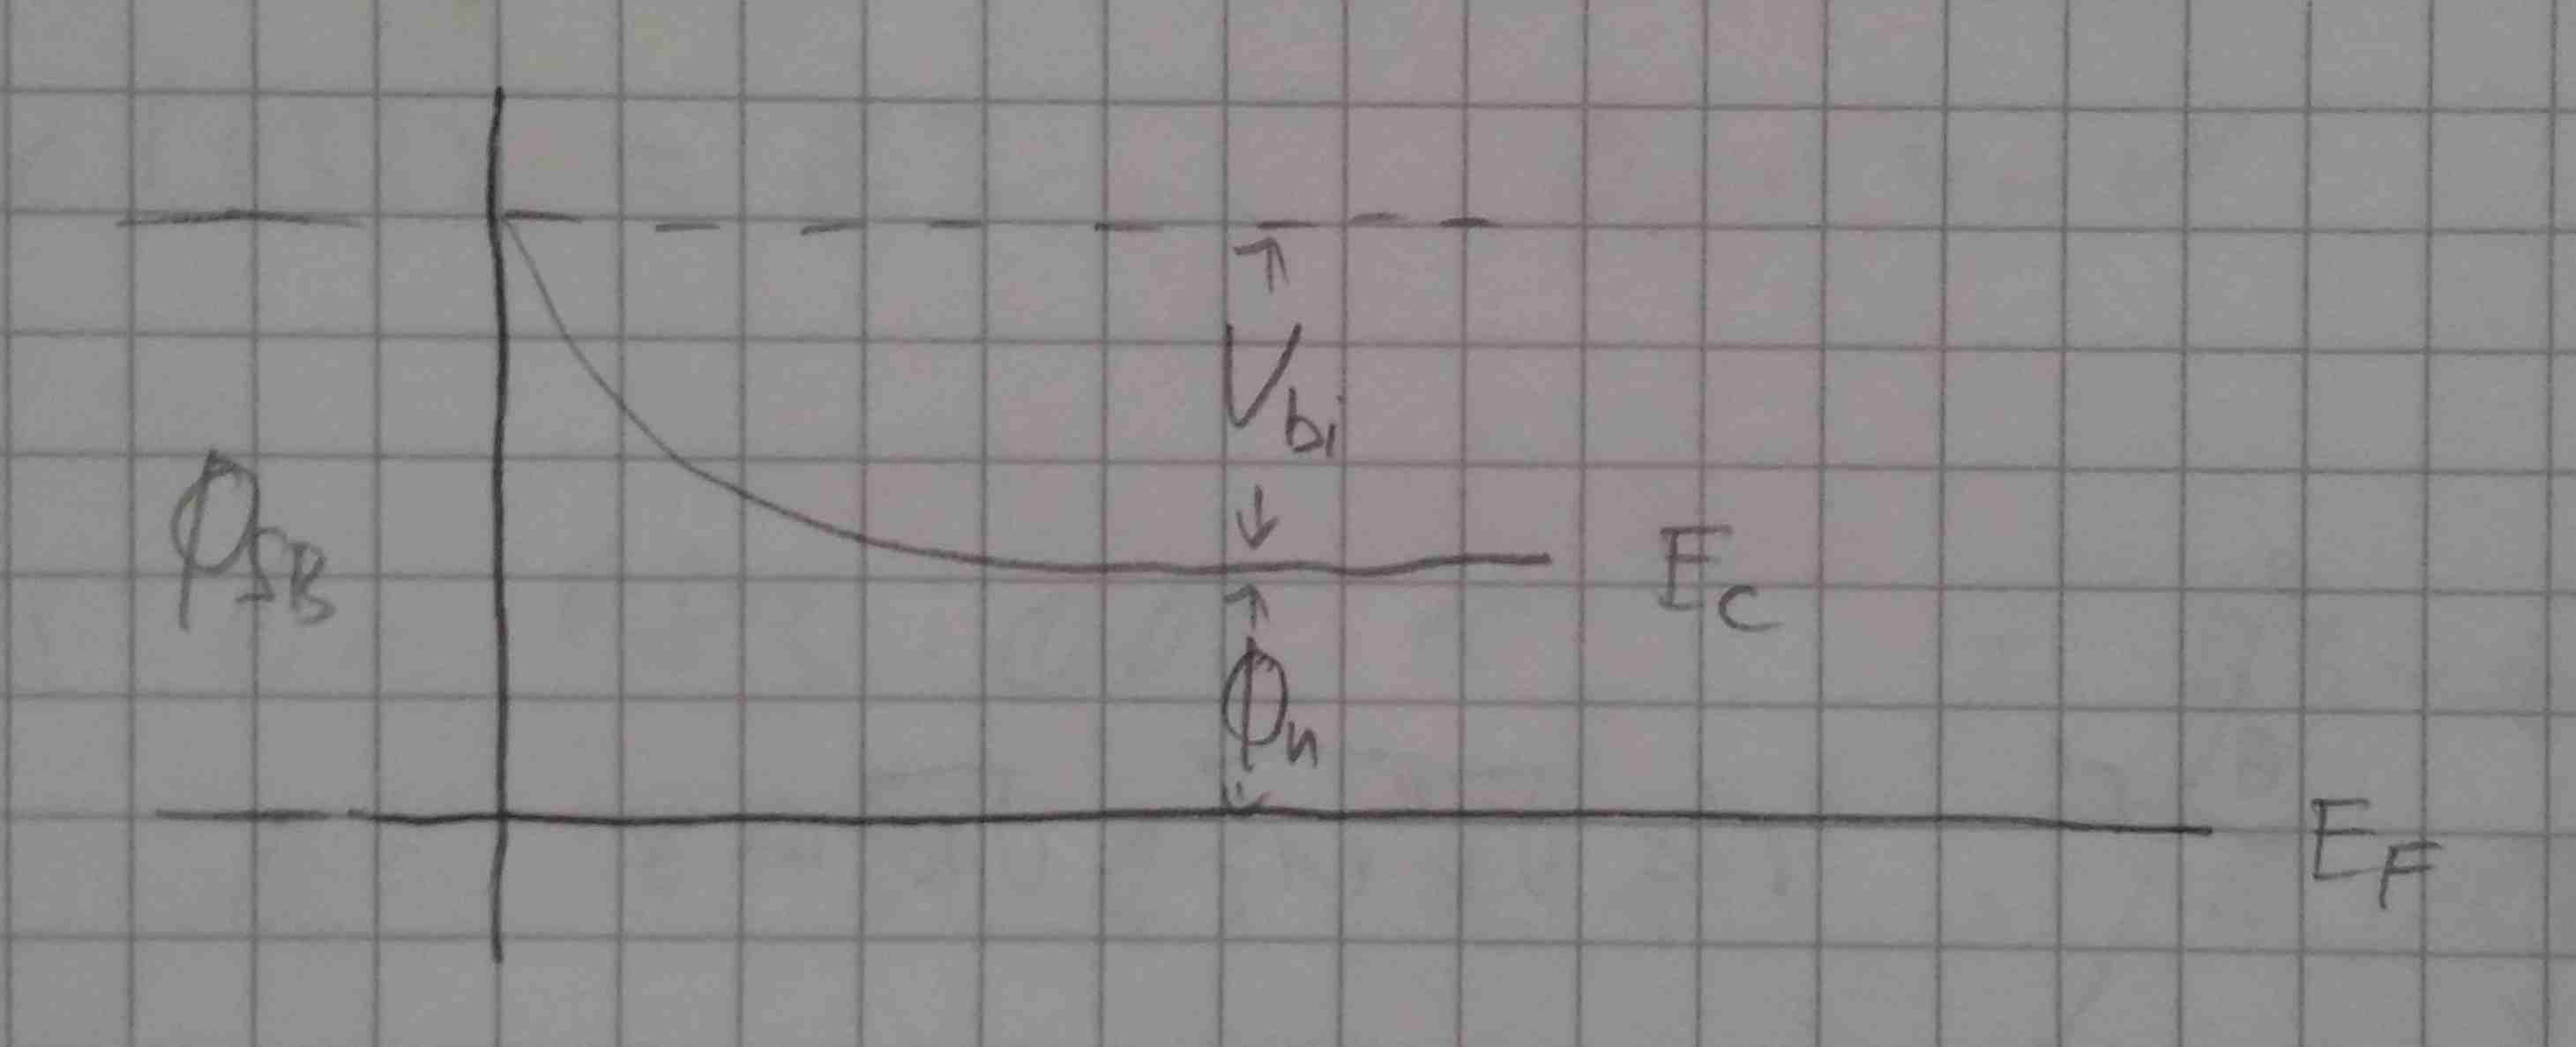
\includegraphics[scale=0.1]{A1_1.jpg}
\end{figure}

Pinch-Off Spannung heißt, das die Raumladungszone verarmt ist. Diese Spannung können wir so berechnen:

\begin{align*}
V_P &= \frac{a^2 e N_d}{2 \cdot \epsilon_0 \cdot \epsilon_r} = \frac{\left( 400 \cdot 10^{-9} \right)^2 \cdot 1,6 \cdot 10^{-19} \cdot 10^{23}}{2 \cdot 8,85 \cdot 10^{-12} \cdot 12,9} = \unit[11,2]{V}
\end{align*}


\subsection*{b)}

\begin{align*}
I_{Sä} &= I_P \cdot \left[ \frac{3 \cdot \left( V_P - V_g - V_{bi} \right)}{V_P} - \frac{2 \cdot \left( V_P^{3/2} - \left( V_g + V_{bi} \right)^{3/2} \right)}{V_P^{3/2}} \right]
\intertext{Dabei ist der Pinch-Off Strom:}
I_P &= \frac{z \cdot \mu \cdot q^2 \cdot N_d^2 \cdot a^3}{6 \cdot \epsilon_0 \epsilon_r \cdot L} = \frac{30 \cdot 10^{-6} \cdot 0,2 \cdot \left( 1,6 \cdot 10^{-19} \right)^2 \cdot \left( 10^{23} \right)^2 \cdot \left( 400 \cdot 10^{-9} \right)^3}{6 \cdot 8,85 \cdot 10^{-12} \cdot 12,9 \cdot 3 \cdot 10^{-6}} = \unit[47,8]{mA}
\intertext{Die Sättigungsspannungen sind dann:}
I_{V_g = 2} &= 47,8 \cdot \left[ \frac{3 \cdot \left( 11,2 - 2 - 0,6 \right)}{11,2} - \frac{2 \cdot \left( 11,2^{3/2} - \left( 2 + 0,6 \right)^{3/2} \right)}{11,2^{3/2}} \right] = \unit[25,2]{mA} \\
I_{V_g = 4} &= 47,8 \cdot \left[ \frac{3 \cdot \left( 11,2 - 4 - 0,6 \right)}{11,2} - \frac{2 \cdot \left( 11,2^{3/2} - \left( 4 + 0,6 \right)^{3/2} \right)}{11,2^{3/2}} \right] = \unit[14]{mA} \\
I_{V_g = 6} &= 47,8 \cdot \left[ \frac{3 \cdot \left( 11,2 - 6 - 0,6 \right)}{11,2} - \frac{2 \cdot \left( 11,2^{3/2} - \left( 6 + 0,6 \right)^{3/2} \right)}{11,2^{3/2}} \right] = \unit[6]{mA} 
\end{align*}

\subsection*{c)}

Die Drainströme werden bei folgenden Spannungen erreicht:

\begin{align*}
V_{DS} &= V_P - V_{bi} - V_g \\
\hfil \\
V_{DS,2} &= 11,2 - 0,6 - 2 = \unit[8,6]{V} \\
V_{DS,4} &= 11,2 - 0,6 - 4 = \unit[6,6]{V} \\
V_{DS,6} &= 11,2 - 0,6 - 6 = \unit[4,6]{V} \\
\end{align*}


\subsection*{d)}

\begin{figure}[h]
	\centering
	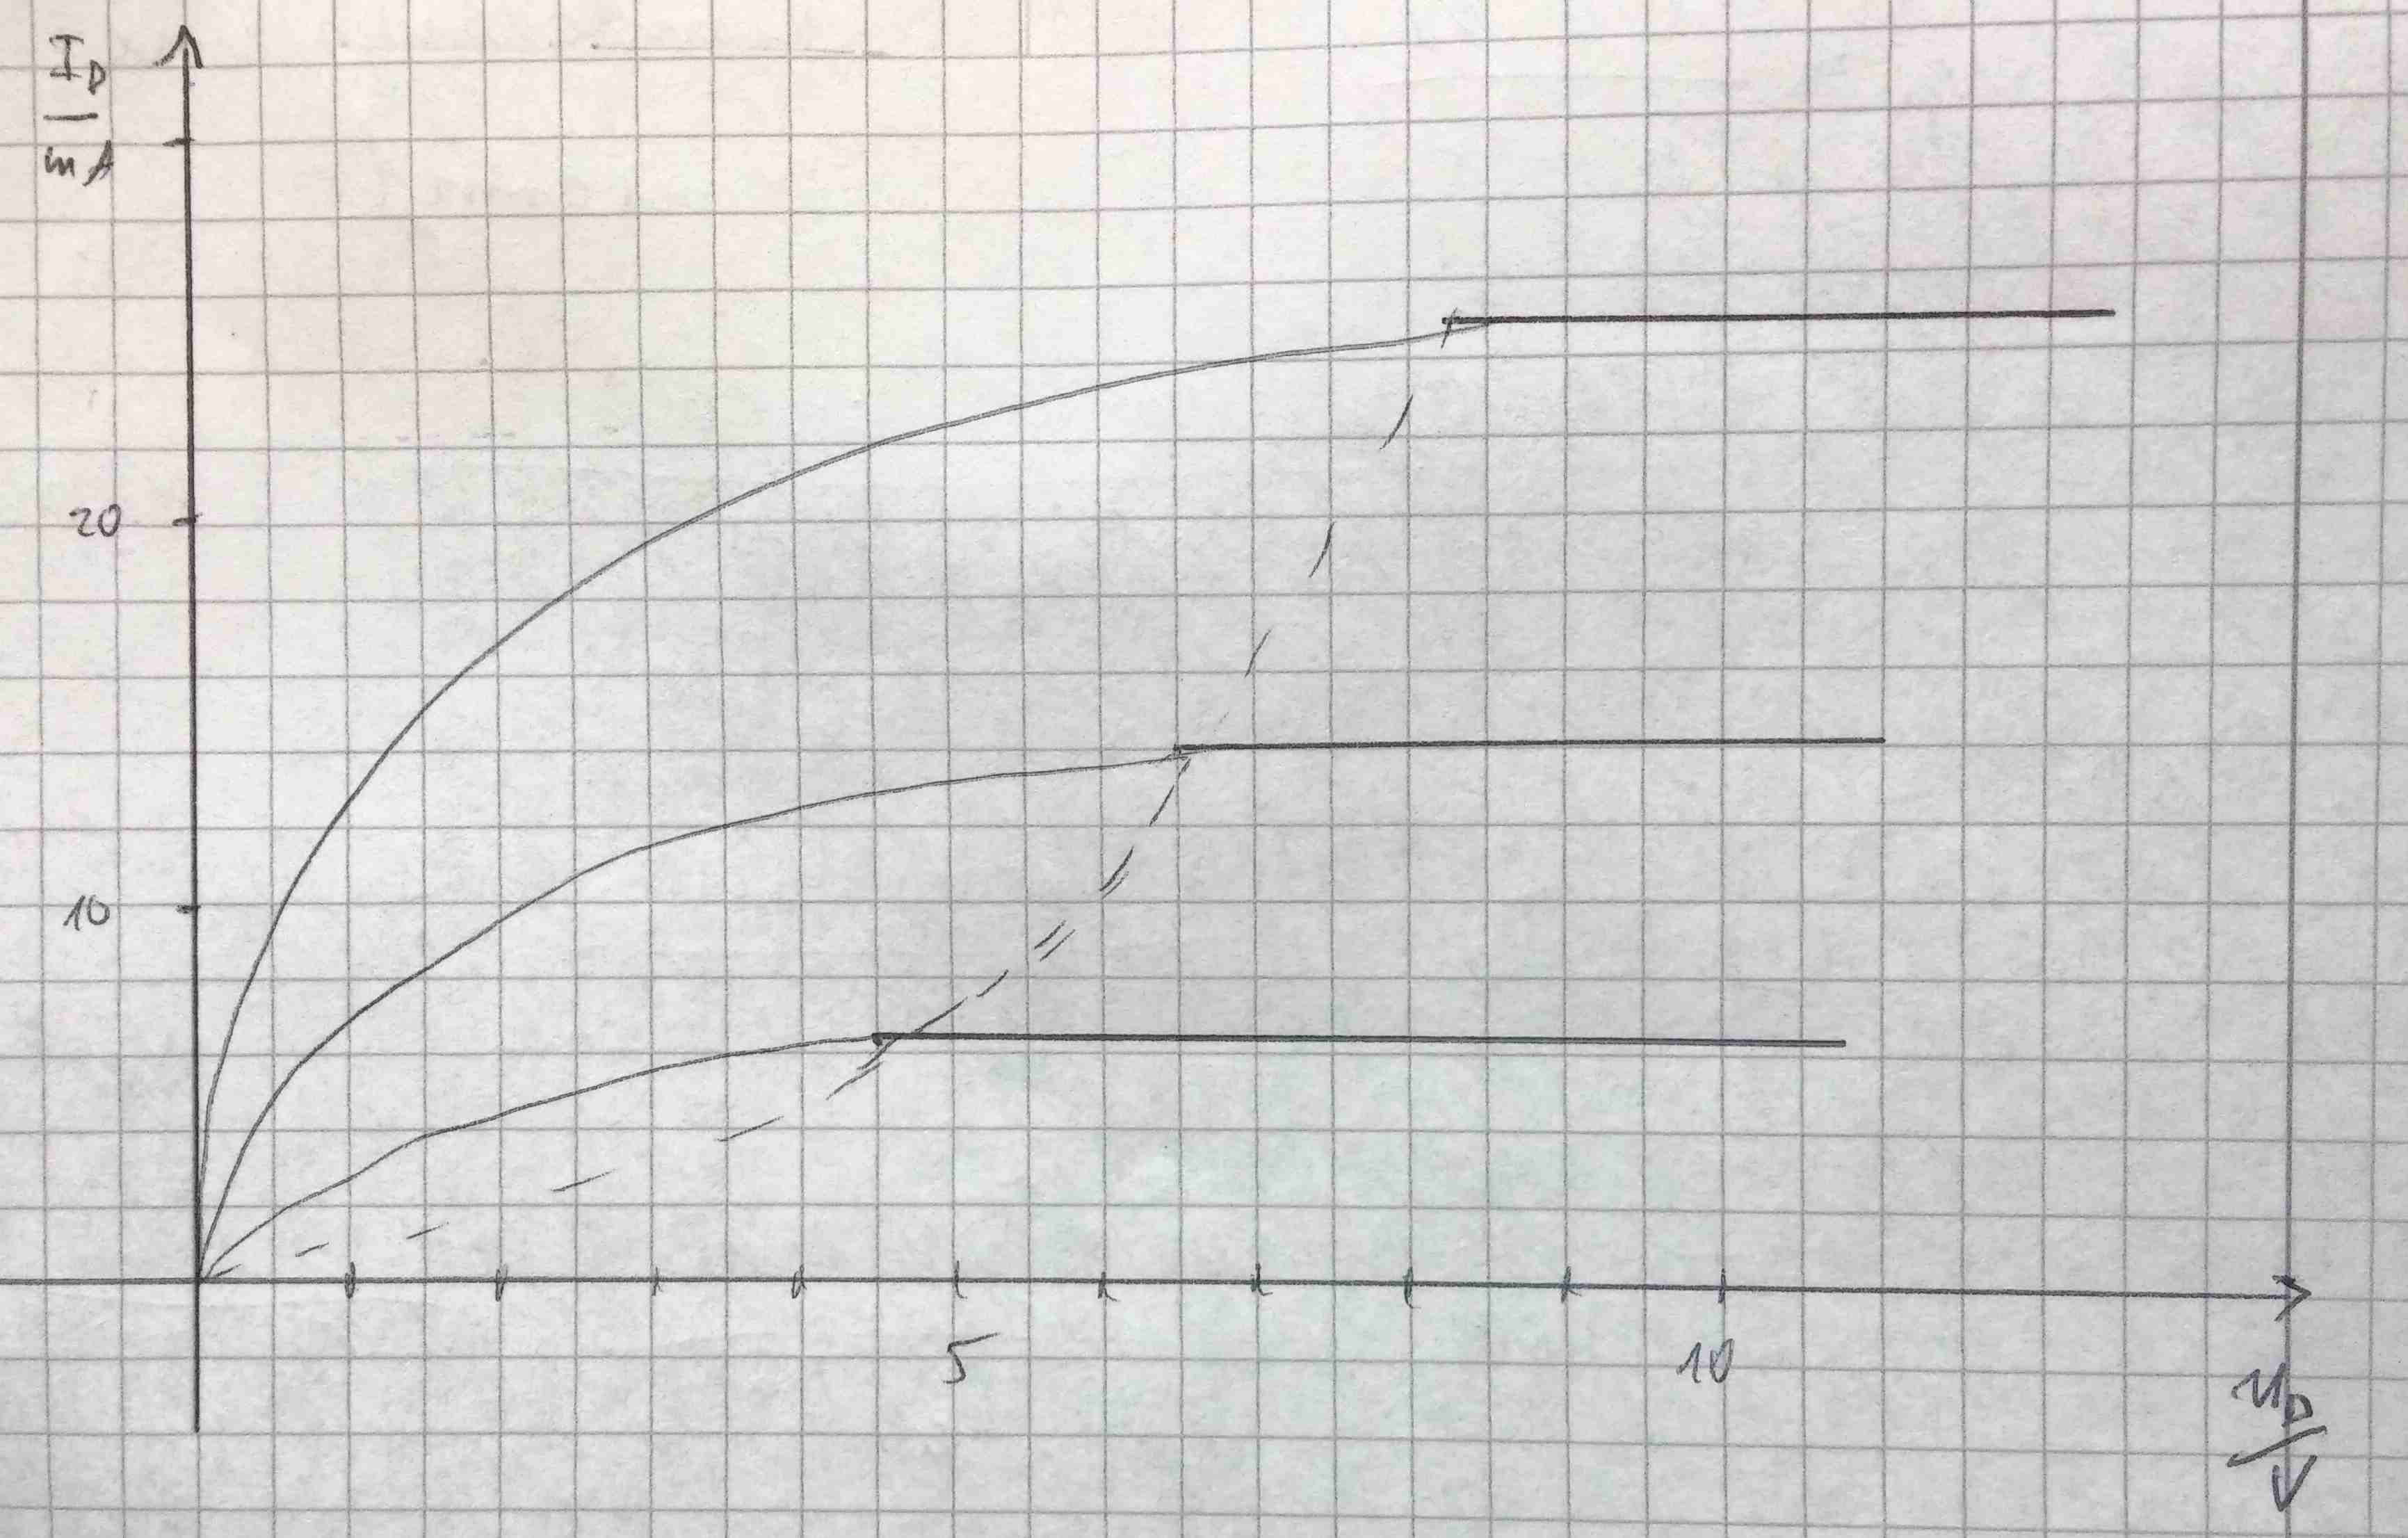
\includegraphics[scale=0.1]{A1_2.jpg}
\end{figure}


\subsection*{e)}

Die Steilheiten können wir wieder mit einer Formel berechnen:

\begin{align*}
-g_{m,2} &= I_P \cdot \left[ \frac{-3}{V_P} + \frac{3 \cdot \sqrt{V_g + V_{bi}}}{V_P^{3/2}} \right] = 47,8 \cdot \left[ \frac{-3}{11,2} + \frac{3 \cdot \sqrt{2 + 0,6}}{11,2^{3/2}} \right] = \unit[6,6]{mA/V} \\
-g_{m,4} &= 47,8 \cdot \left[ \frac{-3}{11,2} + \frac{3 \cdot \sqrt{4 + 0,6}}{11,2^{3/2}} \right] = \unit[4,6]{mA/V} \\
-g_{m,2} &=  47,8 \cdot \left[ \frac{-3}{11,2} + \frac{3 \cdot \sqrt{4 + 0,6}}{11,2^{3/2}} \right] = \unit[2,8]{mA/V}
\end{align*}


\newpage

\section{Aufgabe 2}

\subsection*{a)}

\begin{figure}[h]
	\centering
	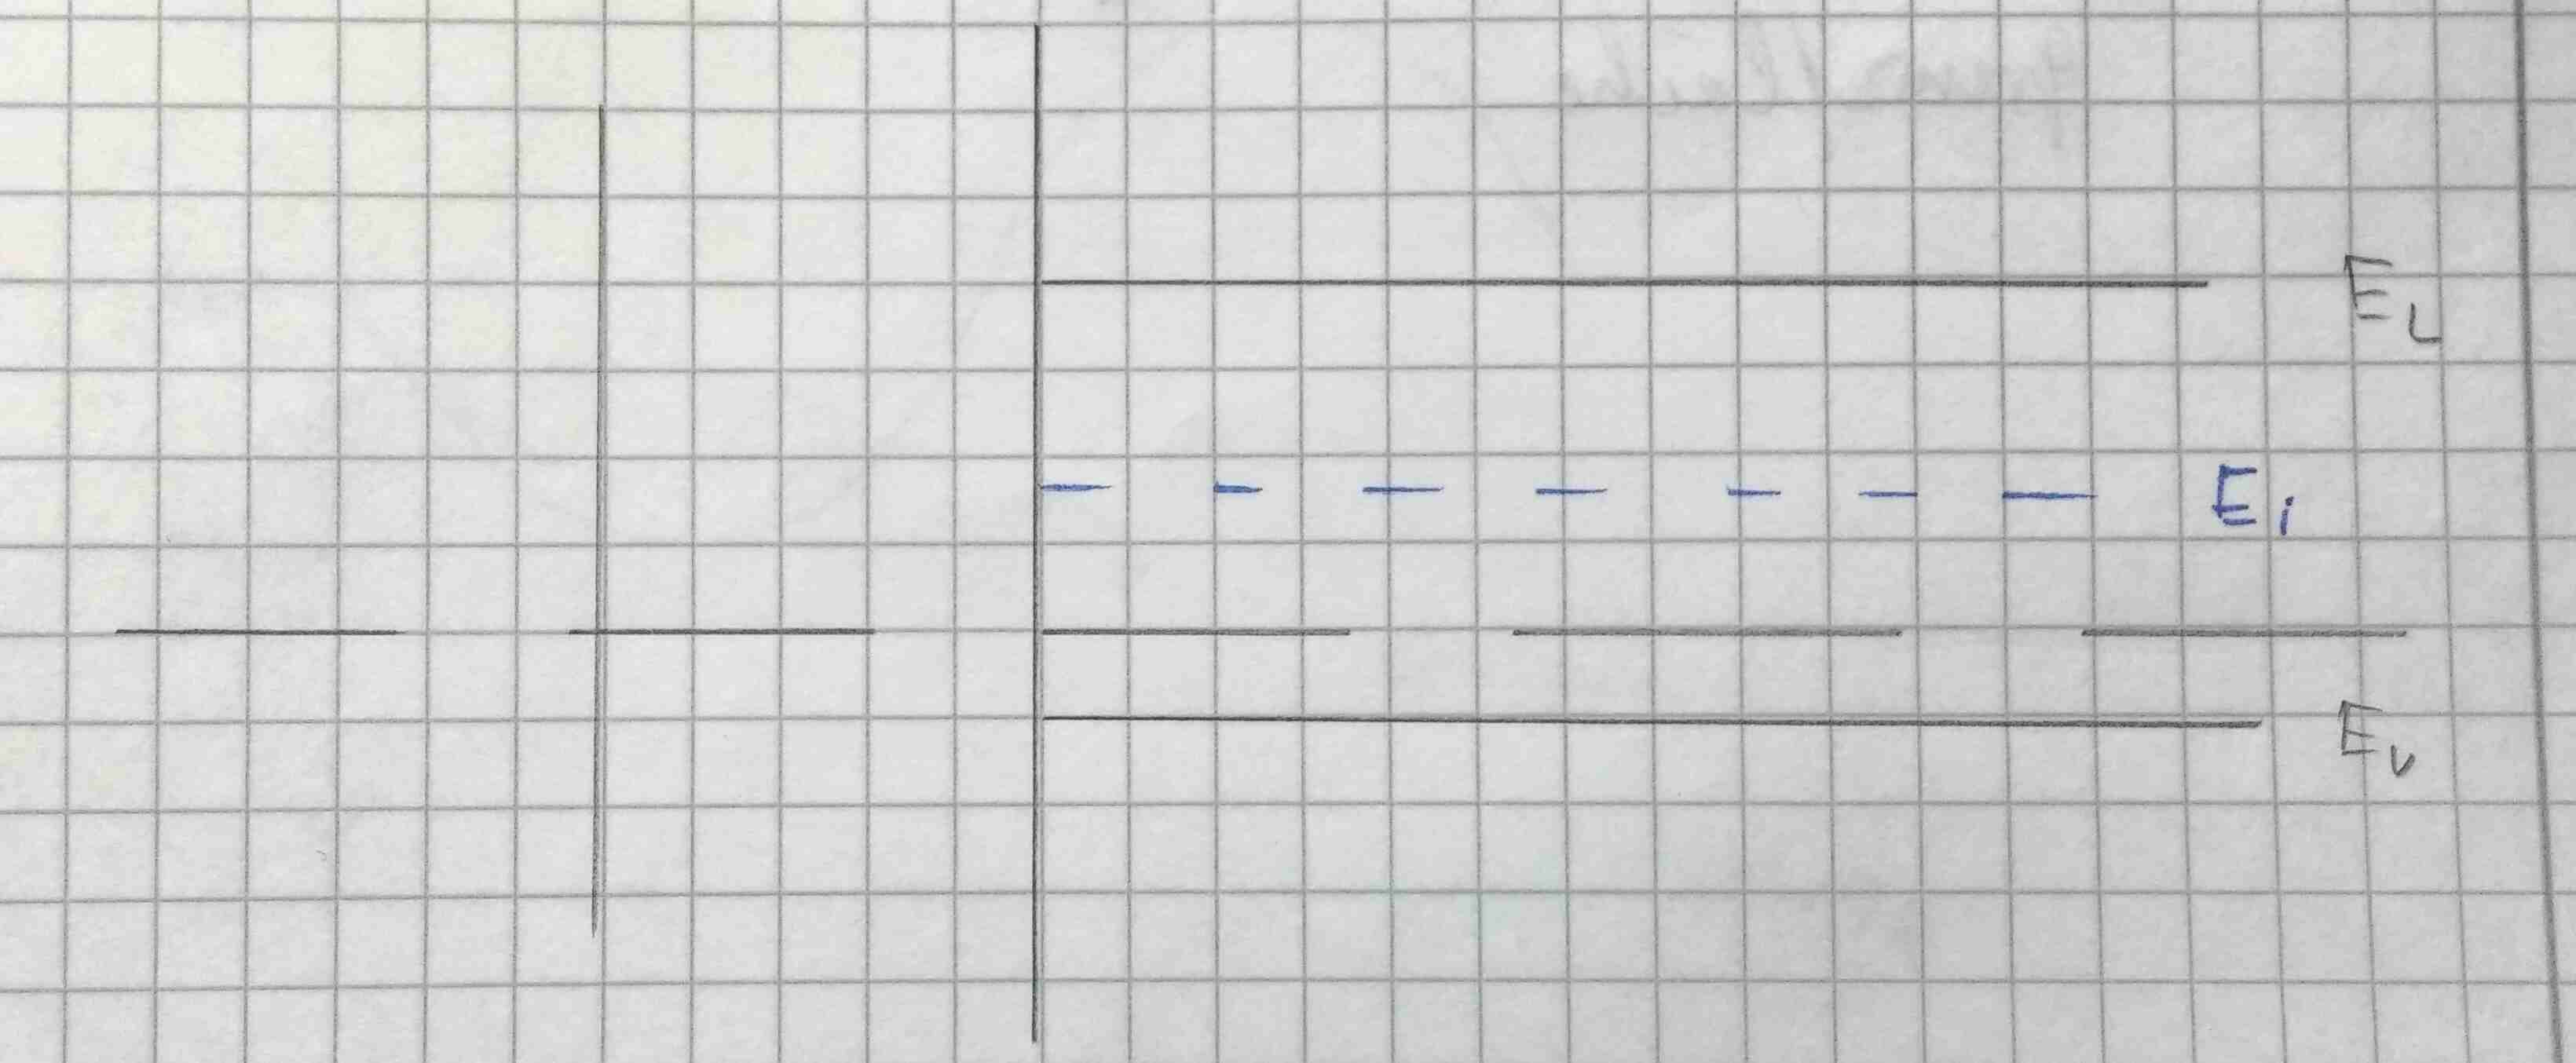
\includegraphics[scale=0.13]{A2_1.jpg}
\end{figure}


\subsection*{b)}

\begin{figure}[h]
	\centering
	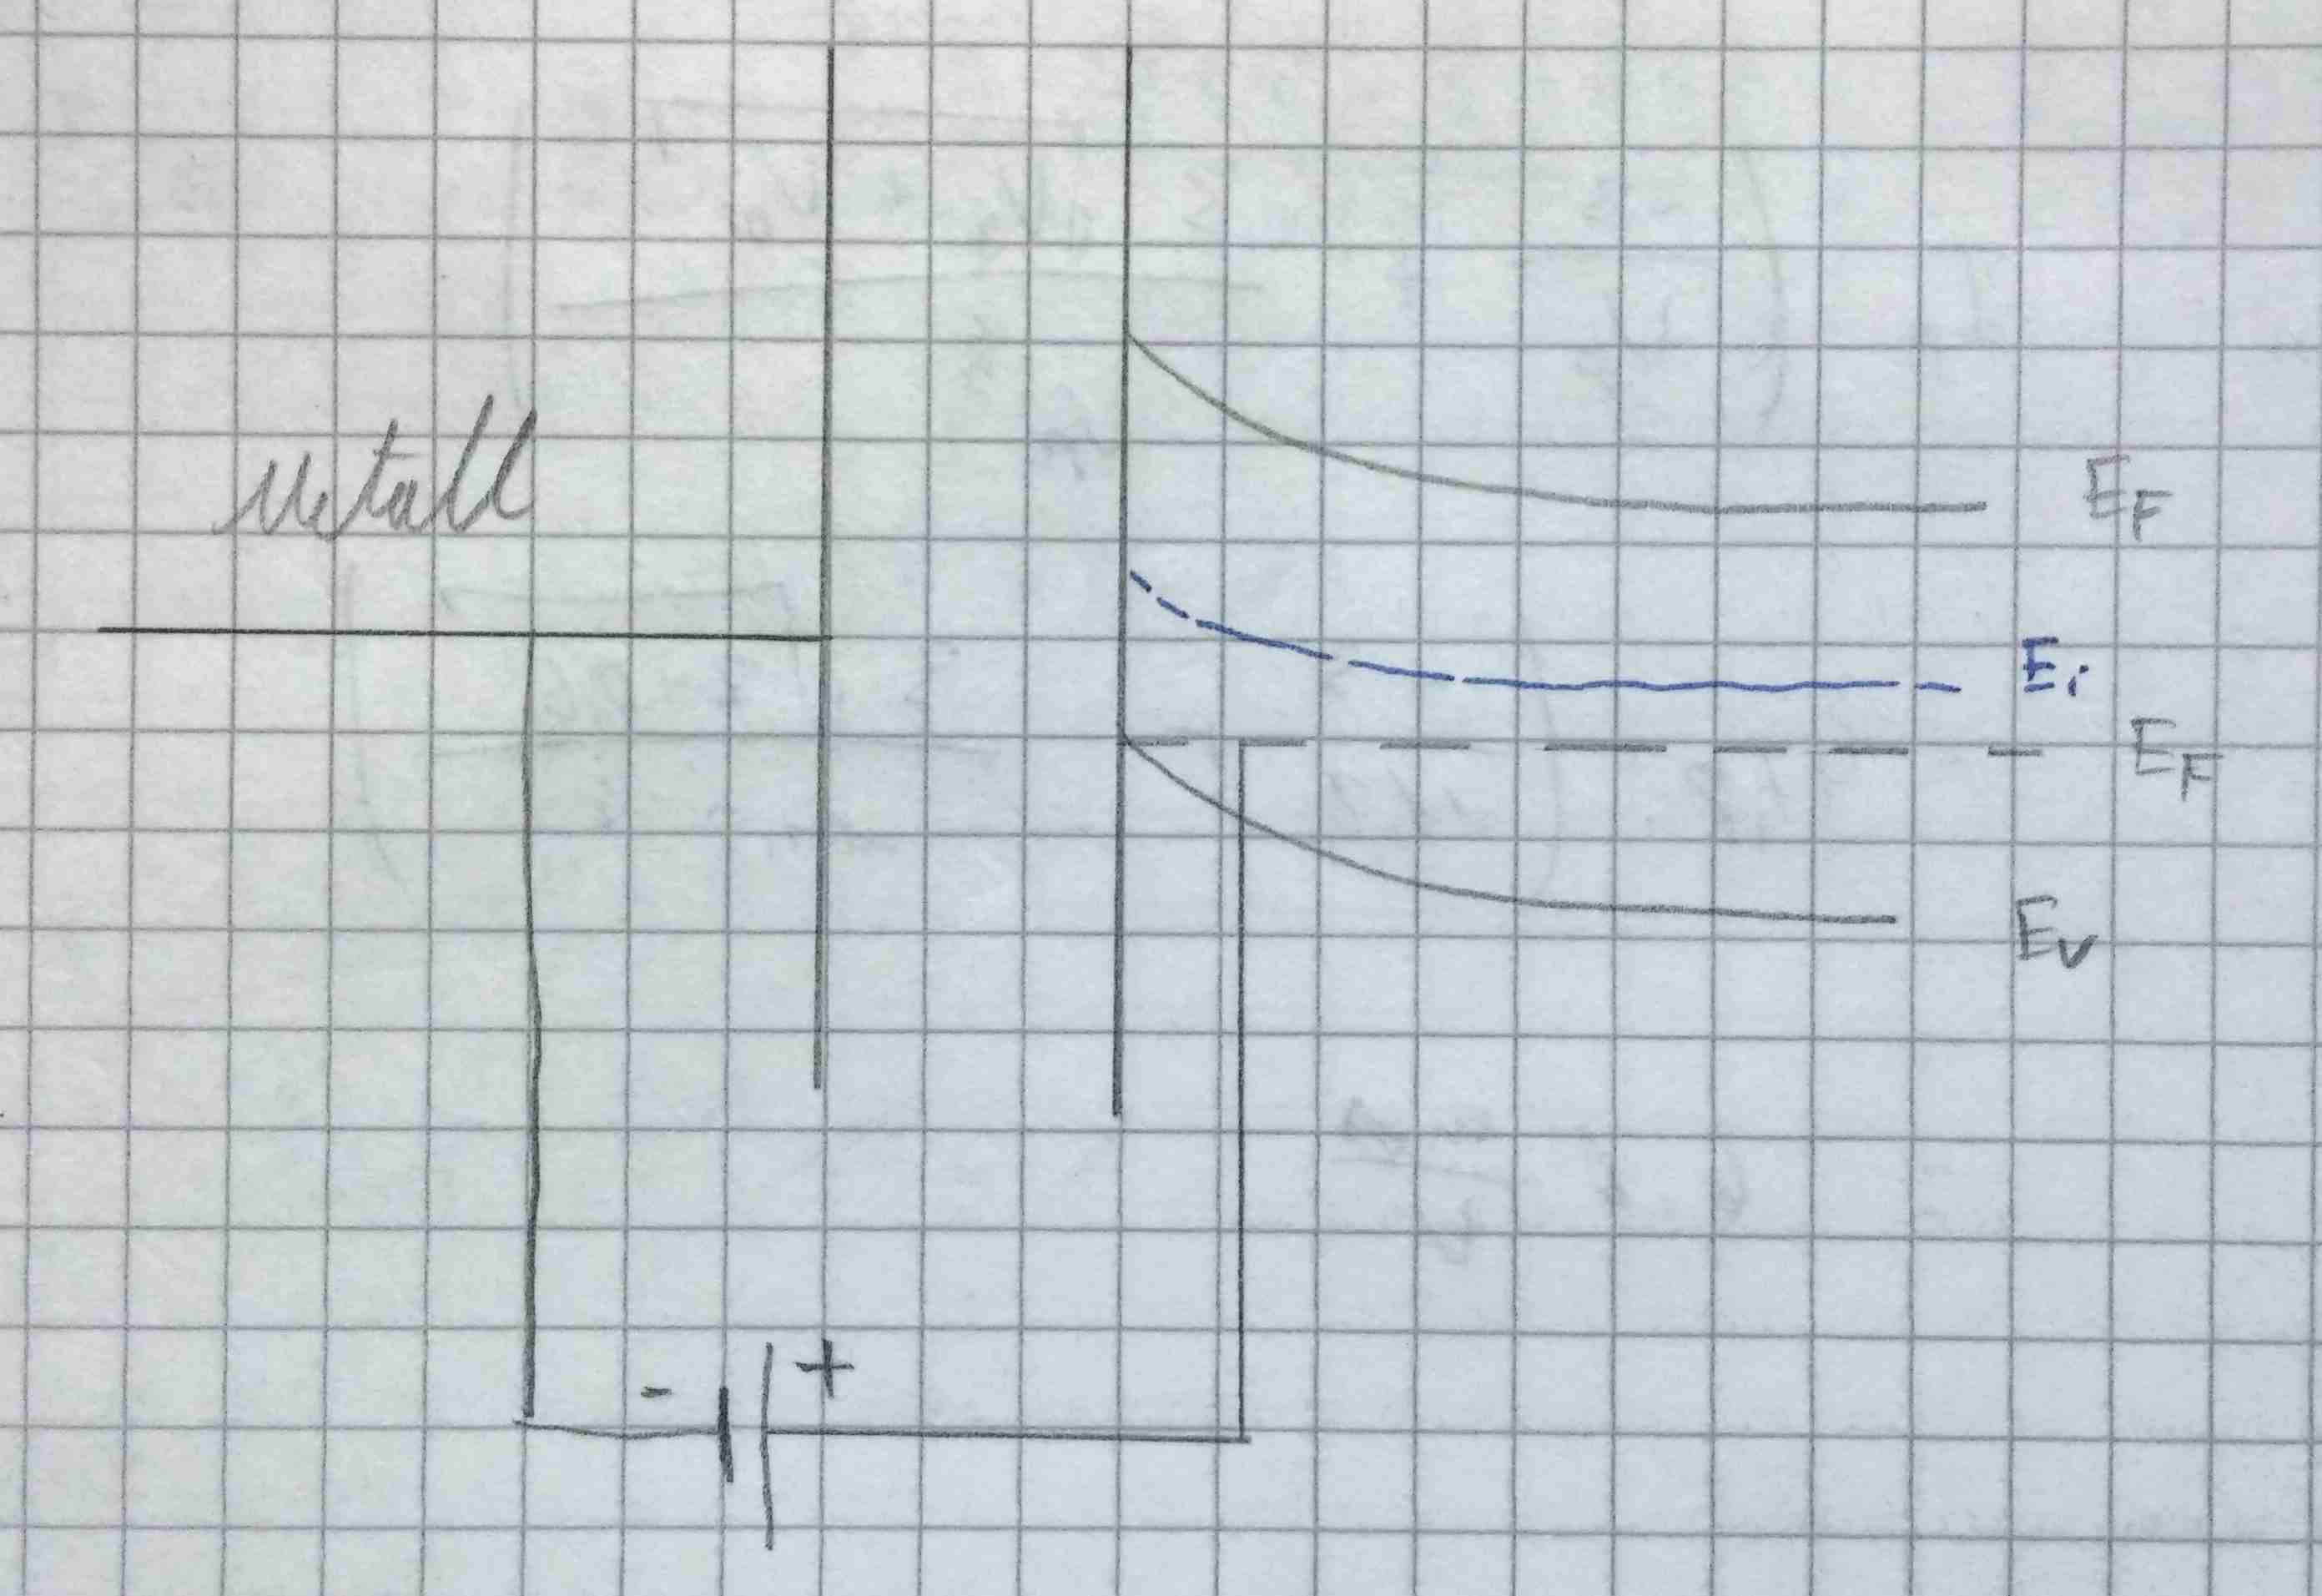
\includegraphics[scale=0.13]{A2_2.jpg}
\end{figure}


\newpage

\subsection*{c)}

\begin{figure}[h]
	\centering
	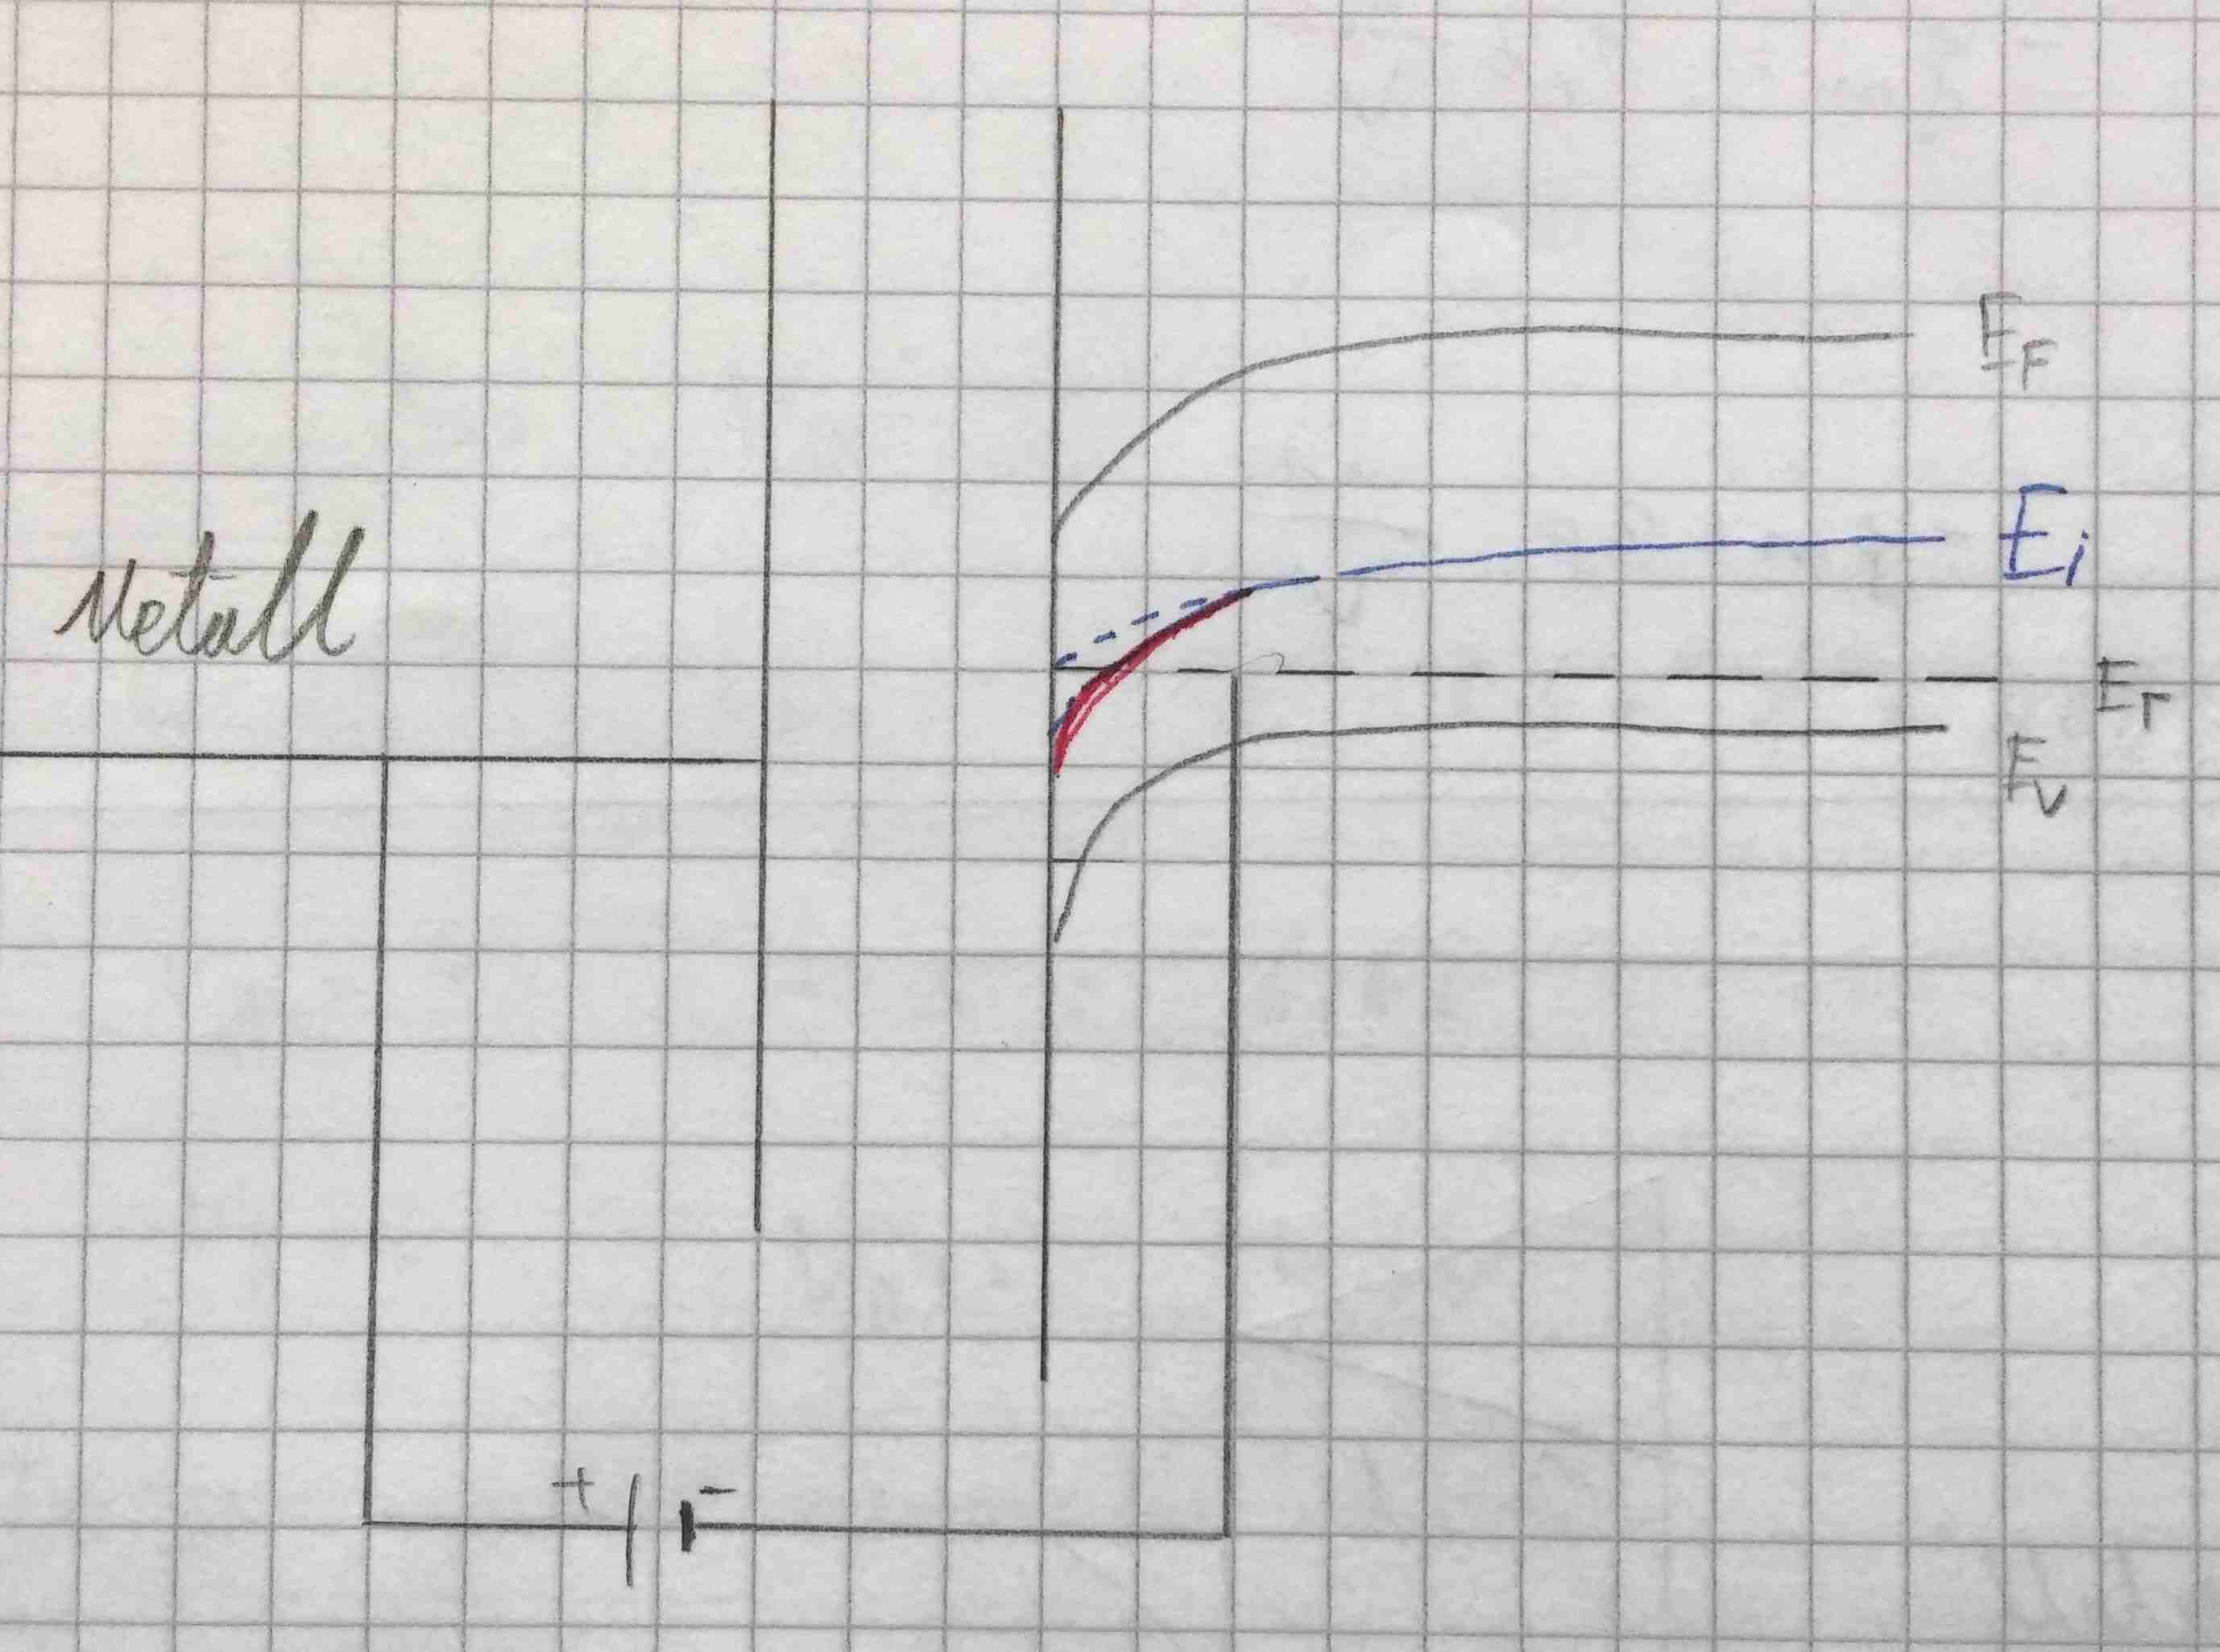
\includegraphics[scale=0.13]{A2_3.jpg}
\end{figure}

Wenn wir noch höhere Spannungen anlegen, dann kommt es zur Invresion an der Grenzfläche. Das ist n-Leitung und in \textcolor{red}{rot} gekennzeichnet.



\section{Aufgabe 3}

\subsection*{a)}

\begin{figure}[h]
	\centering
	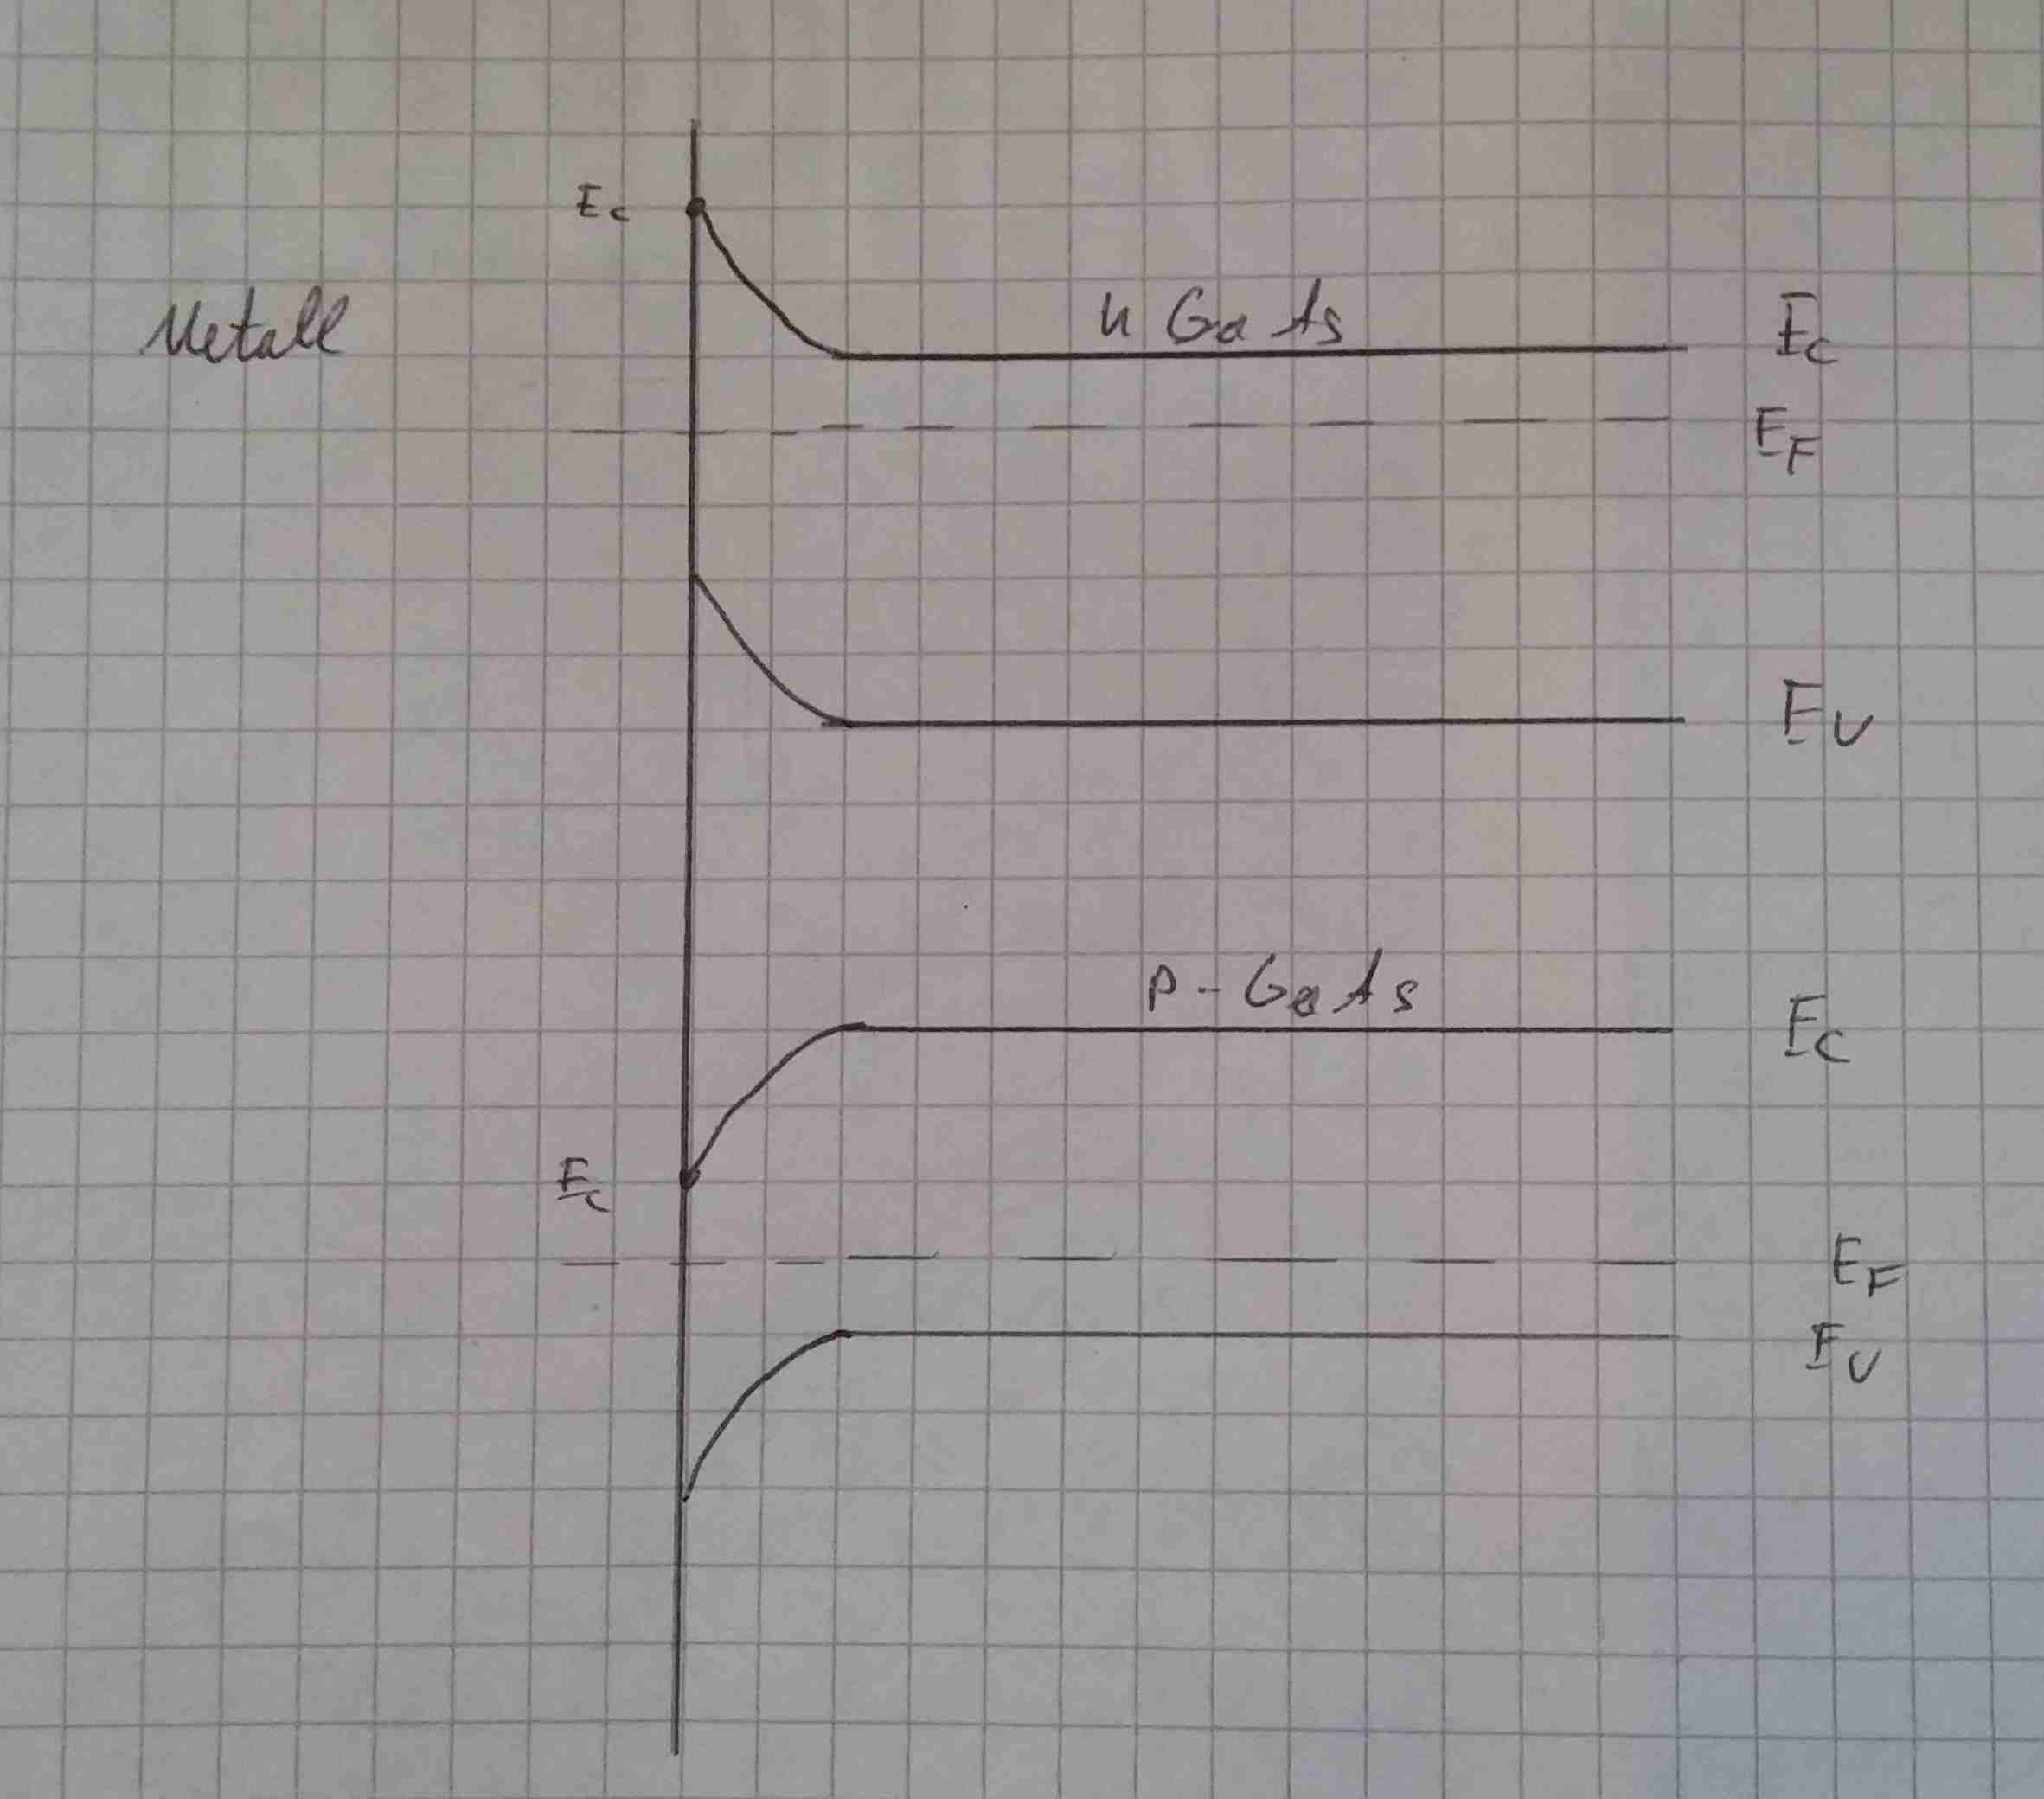
\includegraphics[scale=0.13]{A3_1.jpg}
	\caption{Arbeitsgrade mit Ausgangsspannung in grün}
\end{figure}


Die Spannung am Lastwiderstand bestimmen wir über das ohmsche Gesetz:

\begin{align*}
U_L &= R_L \cdot I_L = 250 \cdot 25 \cdot 10^{-3} = \unit[6,25]{V}
\intertext{Damit fällt für die Ausgangsspannung noch ab:}
U_{out} &= 20 - 6,25 = \unit[13,75]{V}
\end{align*}



\subsection*{b)}

in grün im ersten Bild.

\subsection*{c)}


\begin{figure}[h]
	\centering
	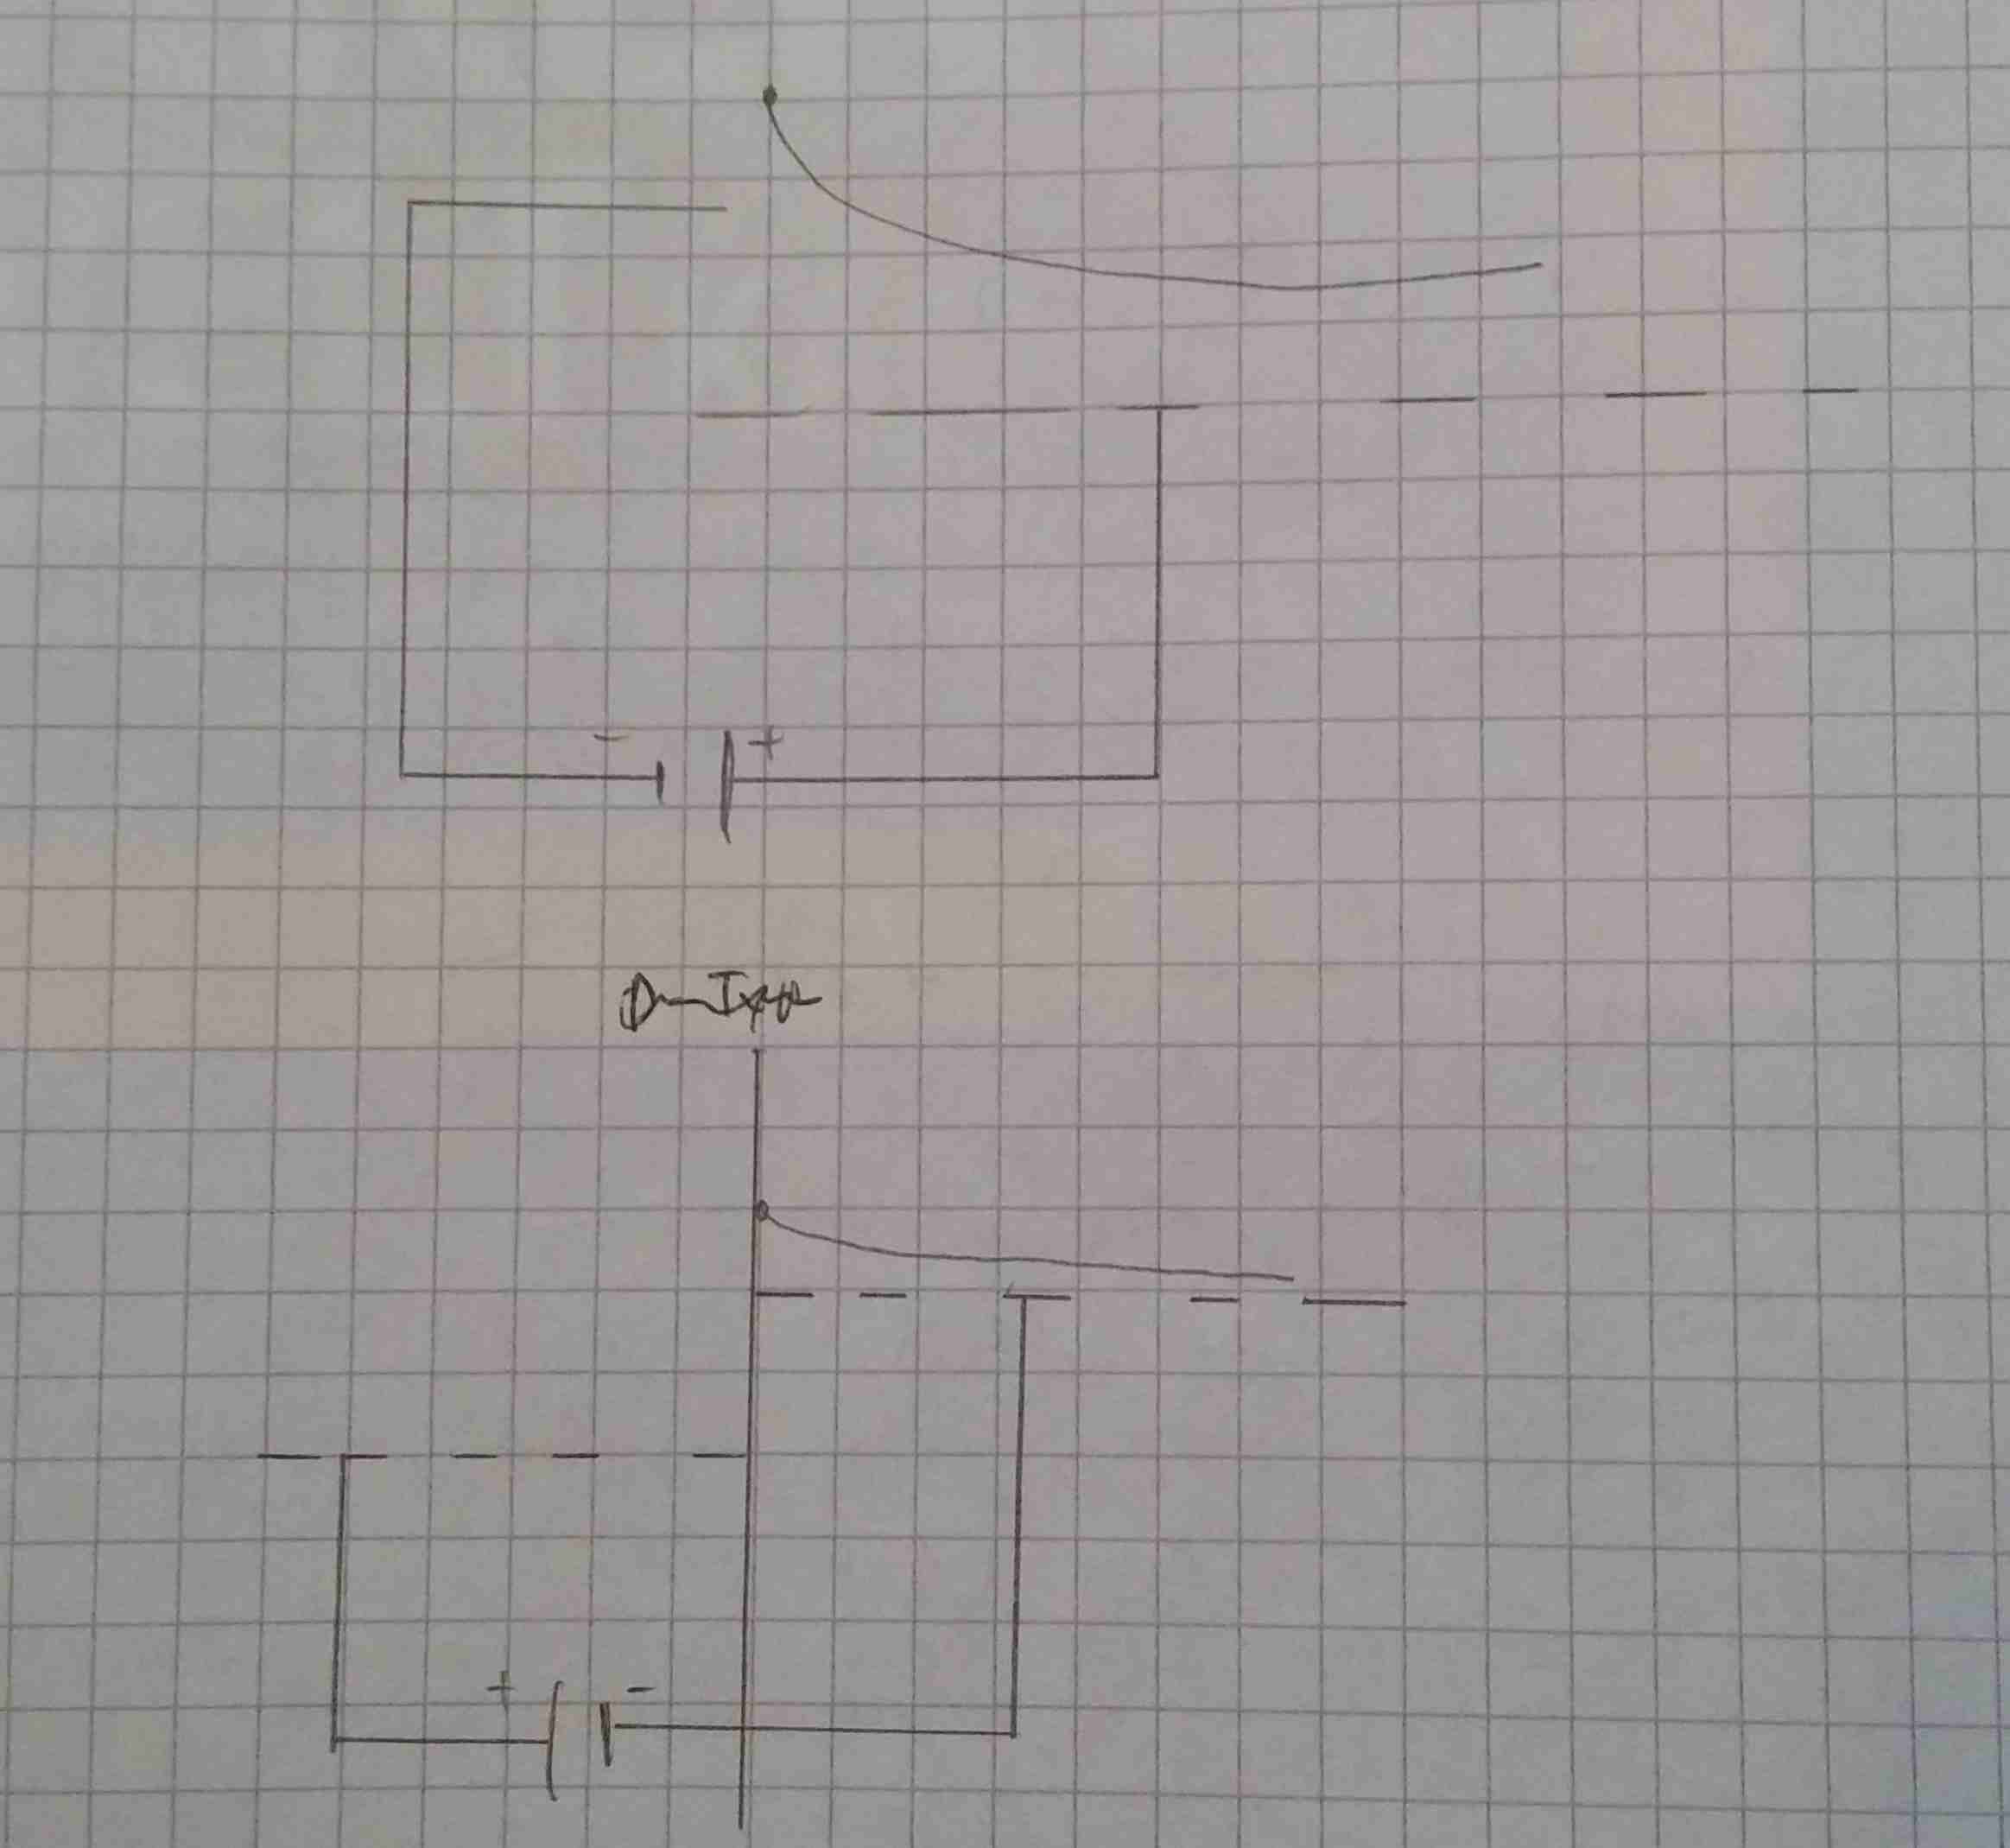
\includegraphics[scale=0.13]{A3_2.jpg}
\end{figure}


\subsection*{d)}

Nein, da hier die negative Halbwelle größer ist als die positive.

\subsection*{e)}

\begin{align*}
\frac{\Delta U_{out}}{\Delta U_{in}} = \frac{3}{1} = 1,5
\end{align*}


\section{Aufgabe 4}

wurde nicht besprochen.












\end{document}